\section{Discrete Time Avoidance}
So far, we've considered that the system is continuous time. 
This is a reasonable expectation, if we have a high sampling time $\Delta t$, compared to the dynamics, i.e., $\| \Delta t \, \dot{\vecs \xi} \| \ll 1$.

However, for the disturbance rejection in the presence of obstacles, a high control force should be exerted to reject the disturbance acceleration (while still remaining within the control robots limits), hence $\| \Delta t \, \vecs \tau^c \| \gg 1$. 
In this case, it is crucial to analyse the discrete time system to guarantee stability (see Figure~
\ref{fig:discrete_controller_parameters_comparison}).

\begin{figure}[htb]
\centering
  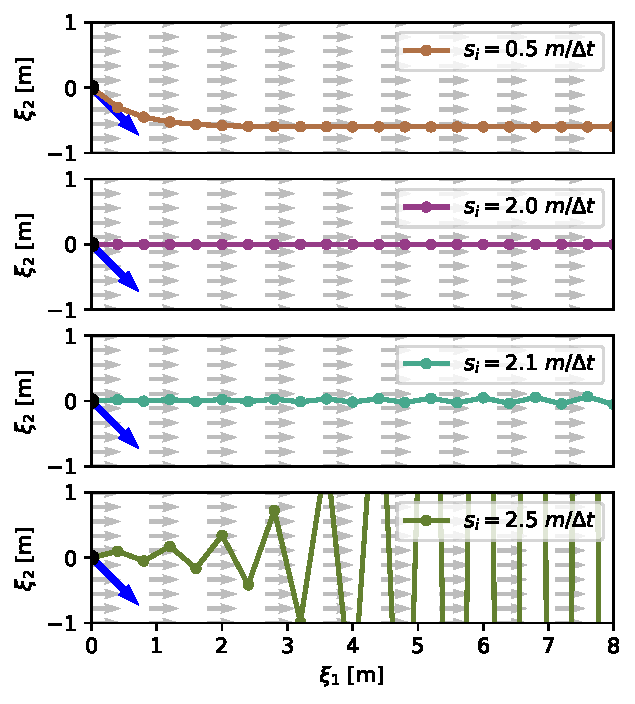
\includegraphics[width=\columnwidth]{figures/discrete_controller_parameters_comparison}
  \caption{A point like agent with initial velocity of $\{ \dot{\vecs \xi} \}_0 = [1 \; -1]^T$ is guided by the dynamics $\vect f(\vecs \xi) = [1, 0]^T$, with equal damping values $s_i$ in all directions, where $m$ is the mass of the agent (the matrix has diagonal form). 
  Damping values above $s_i = 2.0 m / \Delta t$ lead to instable behavior where the higher value leads to higher oscillations. Conversely, the lowest value leads to more deviation from the straight trajectory resulting from the higher impedance. The critical value of $s_i = 2.0 m / \Delta t$ results in stable behavior with immediate correction to the desired velocity.}
  \label{fig:discrete_controller_parameters_comparison}
\end{figure}

 The discrete time case, the state and velocity of the agent evolve as follows:
\begin{equation}
	\begin{bmatrix}
	 \vecs \xi_{t+1} \\ \dot{\vecs \xi}_{t+1}
	\end{bmatrix}
	=
	\begin{bmatrix}
	 \vecs \xi_{t} \\ \dot{\vecs \xi}_{t}
	\end{bmatrix}
	+ 
	\Delta t 
	\begin{bmatrix}
		\dot{\vecs \xi}_{t} \\ \ddot{\vecs \xi}_t 
	\end{bmatrix}
	\eqref{eq:discrete_time_dynamics}
\end{equation}

\begin{lemma}
	Let us consider a discrete time system given in \eqref{eq:discrete_time_dynamics}, which is governed by the controller define in \eqref{eq:damping_summation}.
	with starting velocity $\dot{\vecs \xi}_0 \in \mathbb{R}^N$ such that $\| \dot{\vecs \xi}_0\| \leq v^{\mathrm{max}}$ and a discrete time evolution given by \eqref{eq:discrete_time_dynamics}. The system's velocity is bounded for all t 
\end{lemma}

\begin{proof}
For the algorithm applied in discrete time, as will be the case for any digital controller, the evolution of the velocity is given by:
\begin{equation}
	\begin{split}
	& \begin{bmatrix}
	 \vecs \xi_{t+1} \\ \dot{\vecs \xi}_{t+1}
	\end{bmatrix}
	=
	\begin{bmatrix}
		\vect \xi_t + \Delta t  \; \dot{\vect \xi}_t \\ \
		\dot{\vecs \xi}_t + \Delta t \, \matd{M}^{-1} \matd{D} \left( \vect f(\vecs \xi_t) - \dot{\vecs \xi}_t \right)
	\end{bmatrix} \\
	&  =
	\begin{bmatrix}
		1 & \Delta t \\
		0 & 1 - \Delta t \matd{M}^{-1} \matd D 
	\end{bmatrix}
	\begin{bmatrix}
		\vect \xi_t \\ \dot{\vect \xi}_t
	\end{bmatrix}
	+ \begin{bmatrix}
		0 \\ 
		\Delta t \, \matd{M}^{-1} \matd{D} \vect f(\vecs \xi_t) 
	\end{bmatrix} \\
	& \approx 
	\begin{bmatrix}
		1 & \Delta t \\
		\Delta t \matd{M}^{-1} \matd D \frac{\partial \vect f}{\partial \vecs \xi} & 1 - \Delta t \matd{M}^{-1} \matd D 
	\end{bmatrix}
	\begin{bmatrix}
		\vect \xi_t \\ \dot{\vect \xi}_t
	\end{bmatrix}
	\label{eq:discrete_time_proof}
	\end{split}
\end{equation}

% Let us introduce the coordinate transform $\dot{\vect \gamma}_t = \dot{\vect \xi}_t - \vect f(\vecs \xi)$  and hence for the position we have $\vect \gamma_t = \vect \xi_t - \Delta t \vect f(\vecs \xi)$, and hence 
% \begin{equation}
% 	\begin{split}
% 		\begin{bmatrix}
% 			\vect \gamma_{t+1} \\ \dot{\vect \gamma}_{t+1}
% 						\end{bmatrix}
% 	& =	
% 	\begin{bmatrix}
% 		1 & \Delta t \\
% 		0 & 1 - \Delta t \, \matd{M}^{-1} \matd{D}
% 	\end{bmatrix}
% 	\begin{bmatrix}
% 		\vecs \gamma_t \\ \dot{\vecs \gamma}_t
% 	\end{bmatrix}
% 	+ \begin{bmatrix} 
% 	\Delta t \vect f(\vecs \xi_t) \\ 0
%     \end{bmatrix} \\
% 	& \approx \begin{bmatrix}
% 		1 + \Delta t \frac{\partial \vect f}{\partial \vect \xi} & \Delta t \\
% 		0 & 1 - \Delta t \, \matd{M}^{-1} \matd{D}
% 	\end{bmatrix}
% 	\end{split}
% \end{equation}
The summand $\vect t \vect f(\vecs \xi_t)$ changes the relative position value $\vect \gamma_t$ as long as the desired velocity is not zero. However, this only moves the relative position, but does not influence kinetic energy, which has been used as the stability function (Section~\ref{sec:passivity_analysis}).

Hence, we look at the closed loop system. From which the eigenvalues can be calculated as:
\begin{equation}
	\vect \lambda_1 = 1 \qquad \vect \lambda_2 = 1 - \Delta t \, \matd{M}^{-1} \matd{D}
\end{equation}
Hence, if the eigenvalues are smaller or equal to one, the system is stable. This is the case, if the maximum eigenvalue of $\Delta t \, \matd{M}^{-1} \matd{D} \leq 2$.
\end{proof}

The stability with different damping values can be observed in Figure~\ref{fig:discrete_controller_parameters_comparison}.


\subsection{Asymptotic Stability}
For a general nonlinear system no asymptotic convergence evaluation can be made. This is due to the fact, that for any system there is a slight drift due to the damping values.
And hence, if there are high nonlinearities in the system it could happen that even with a stable system, the dynamics get caught in a limit cycle. However, for most common globally asymptotic systems (for velocity-position), the force controller as proposed leads to globally asymptoticly stable behavior, too (Figure~\ref{fig:discrete_controller_parameters_comparison_stable}).

\subsection{Intertial Drift}
Let us assume that have strong damping in the direction of the obstacle, i.e., $s^{\mathrm{obs}} / m_i \gg 1$, where $m_i$ with $i = 1, .., N$ represent the eigenvalues of the mass matrix $\matd{M}$. 


\begin{figure}[htb]
\centering
  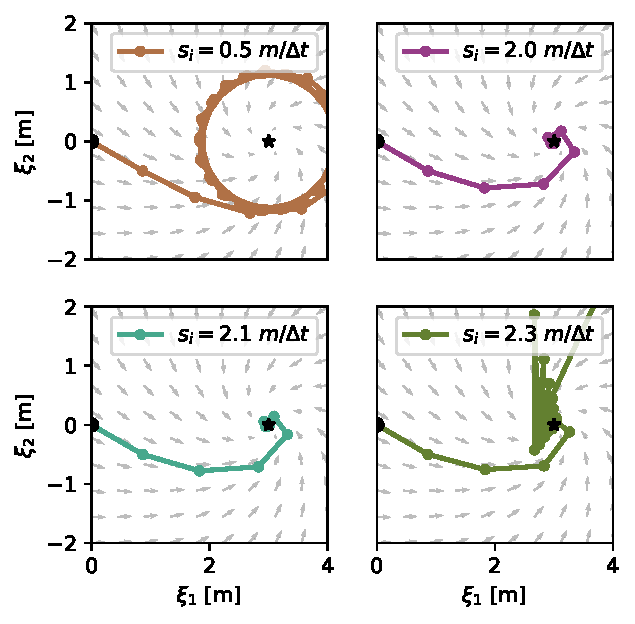
\includegraphics[width=\columnwidth]{figures/discrete_controller_parameters_comparison_stable}
\caption{A point like agent which is following the desired dynamics of
$\vect f(\vecs \xi) = \matr R(\pi / 6) (\vect \xi  - \vect \xi^a)$ where $\matr R(\cdot)$ is the rotation matrix, and with equal damping values $s_i$, where $m$ is the mass of the agent.}
  \label{fig:discrete_controller_parameters_comparison_stable}
\end{figure}

